\documentclass{article}
\usepackage{pgfplots}
\pgfplotsset{compat=1.11}

\begin{document}
\thispagestyle{empty}
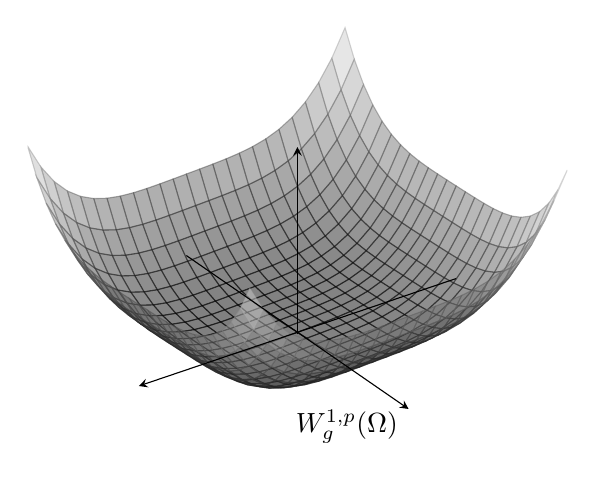
\begin{tikzpicture}
\begin{axis}[view={145}{45},
             axis lines=center,
             axis on top,
             xtick=\empty,ytick=\empty,ztick=\empty,
             xlabel=$W_g^{1,p}(\Omega)$,
             xlabel near ticks,
             xlabel shift={20pt},
             mesh/interior colormap name=blackwhite,
             colormap/blackwhite,]
  \addplot3[domain=-5:5,surf,opacity=0.5]{0.25*abs(x)^4 + 0.25*abs(y)^4 - 2*x + 2*y};
\end{axis}
\end{tikzpicture}
\end{document}

